\documentclass{mpaper}

\usepackage{minted}
\usepackage[numbers]{natbib}
\usepackage[font=bf]{caption}

\providecommand*{\listingautorefname}{Listing}

\setminted{frame=lines, autogobble, breaklines}

\begin{document}

    \title{ptr-tidy: Automatic Rejuvenation of Raw Pointers in C++}
    \author{Artem Usov}
    \matricnum{2296905U}

    \maketitle


%%%%%%%%%%%%%%%%%%%%%%%%%%%%%%%%%%%%%%%%%%%%%%%%%%%%%%%%%%%%%%%%%%%%%%%%%%%%%%%%%%%%%%%%%%%%%%%%%


    \begin{abstract}
    Systems programming involves dynamically requesting memory which in the C++ language has to be manually managed by the programmer. 
    However, this leaves the opportunity for exploitable memory safety errors.
    Modern C++ recommends that smart pointers are used to automatically manage resources such as dynamic memory.
    However, many legacy programs were been written before these features were introduced to the language.
    We develop the ptr-tidy tool in order to automatically rejuvenate such programs to use smart pointers.
    The tool uses the Clang and LLVM libraries in order to create a componentised and powerful framework which could be used by other refactoring or rejuvenation tools. 
    We present a case study and also apply the tool on a number of open-source C++ libraries from a variety of application domains to show that the tool can successfully rejuvenate non-trivial libraries.
    We discuss the circumstances in which the tool performs well and the current limitations.
    \end{abstract}


%%%%%%%%%%%%%%%%%%%%%%%%%%%%%%%%%%%%%%%%%%%%%%%%%%%%%%%%%%%%%%%%%%%%%%%%%%%%%%%%%%%%%%%%%%%%%%%%%


    \section{Introduction}\label{sec:introduction}
    
    Most ordinary computer users demand that the machine they are using provides them with a responsive, secure and productive environment to complete their tasks.
    The programs that are most responsible for this are complex systems programs such as the underlying operating system, device drivers and web browsers.
    Systems programming involves memory management, that is dynamically requesting memory from the operating system to be used and managed by the program.
    This is done as the amount of memory that we need at runtime cannot be known at the time of compilation of the program.
    However, doing so creates the opportunity for memory safety errors~\cite{Dhurjati2003}.
    A memory safety error can be one of:
    \begin{itemize}
        \item \textbf{Dangling pointer}, prematurely freeing memory that is still in use.
        \item \textbf{Double free}, freeing memory multiple times.
        \item \textbf{Never free}, never freeing memory.
    \end{itemize}
    There are other categories of memory safety errors such as buffer overflows which we do not consider in this paper.
    If there are memory safety errors in a program, there is the possibility that it could be exploited by a malicious party to crash the program, expose sensitive data or gain remote code execution capabilities~\cite{Afek2007}.

    Historically, systems programs were mostly written in C, C++ or a combination of the two and these remain the dominant languages.
    They are lower level languages that involve manual memory management by the programmer.
    It is extremely challenging to ensure that C and C++ programs contain no memory safety errors as evidenced by empirical data in industry, where in a presentation at the Linux Security Summit it was shown that in several popular projects such as Firefox, macOS, Ubuntu and Android all had over half of their CVEs~\footnote{\url{https://cve.mitre.org/}} attributed to issues with memory safety~\cite{Gaynor2020}.
    Similarly, in a presentation by Matt Miller, a security engineer at Microsoft, it is shown that around 70\% of their vulnerabilities that are addressed through security updates are due to memory safety issues~\cite{Miller2019}. 
    % This is at industry-leading companies who are renowned for hiring top talent and with top developer education programs.
    
    % However the continued use of C and C++, alongside industry mottos such as \emph{``Move fast and break things''}~\cite{Vardi2018} do not help by possibly diminishing the danger of memory safety error exploitation.
    % However due to new regulations such as the GDPR and increasing oversight by regulators, any such exploitations which do expose sensitive data are more commonly exposed to the general public and punished by regulators.
    % An example is a fine of \pounds20m for a British Airways data breach by the British Information Commissioner's Office~\cite{ICO2020}. 
    
    Unfortunately, simply not using C or C++ is not an option since their unmanaged nature allows for high performance, and therefore the best option for systems with strict or high requirements.
    Engineers at both Microsoft~\cite{Thomas2019} and Mozilla~\cite{Hostfelt2019} converge on Rust~\cite{Balasubramanian2017} as a possible solution.
    Rust is a systems language that offers similar performance as C and C++~\cite{Lin2016}, however its linear type system and memory ownership model guarantee that none of the memory errors that we are considering can occur.
    The rewriting of a program in a new language, namely from C++ to Rust, is a colossal undertaking, especially given that Rust has a reputation for being difficult to learn~\cite{Astrauskas2019}.
    Instead, modern C++ guidelines encourage the use of \emph{smart pointers}~\cite{Dimov2003} and the concept of \emph{RAII (Resource Acquisition Is Initialisation)}~\cite{Stroustrup2000} to create compiler managed resource handles.
    Their correct use eliminates the three previously identified classes of memory safety errors.
    Yet, we encounter further problems as C++ programs either do not actively follow this advice, or are \emph{legacy} programs which were written before these features were introduced to the language.
    
    We therefore propose a solution in the form of a tool, \emph{ptr-tidy}~\cite{Usov2021}, to analyse and automatically refactor programs to follow the recommended use of smart pointers where the analysis can determine that such a change is correct and does not change the runtime behaviour of the program. 
    
    \begin{figure}[t]
        \centering
        \inputminted{c++}{code/leak.cpp}
        
\includegraphics{images/arrow.pdf}
        \inputminted{c++}{code/fix-leak.cpp}
        \caption{Example of a memory leak using manual management and how smart pointers correct this problem. Lines 4 and 5 show how interruptions in the program control flow can mistakenly cause memory leaks as the \texttt{delete} statement is never reached. Smart pointers correct this as the compiler automatically inserts delete statements at all necessary locations at compile time. All necessary headers are omitted for brevity}
        \label{lst:motivating-example}
    \end{figure}
    
    We provide a motivating example in \autoref{lst:motivating-example} where the initial version of the function has several control flow statements that could cause the \texttt{Circle} object to never be freed.
    The example can seem trivial as all the possible executions paths of the program are easy to visualise, but can suddenly become rather non-trivial if the conditions in the \texttt{if} statement become calls into external libraries, which may throw an exception and cause the \texttt{delete} statement to again not be reached.

    
%%%%%%%%%%%%%%%%%%%%%%%%%%%%%%%%%%%%%%%%%%%%%%%%%%%%%%%%%%%%%%%%%%%%%%%%%%%%%%%%%%%%%%%%%%%%%%%%%


    \section{Related Work}\label{sec:related-work}
    
    Our work closely relates to work done around the field of \emph{source code rejuvenation}, as defined by \citet{Pirkelbauer2010}. 
    We exactly aim to replace outdated coding patterns with newer, higher-level abstractions, as well as fitting the notion that this tool would be applied once to a codebase, rather than be a reoccurring task.
    We will however use the terms rejuvenating and refactoring interchangeably in this paper as refactoring is a term that most developers are more familiar with to convey code changes in order to improve the overall quality. 
    
    We believe research in this area is going to increase, as languages move and evolve much quicker than can be supported in enterprise environments~\cite{Overbey2009, Favre2005}, resulting in accumulating technical debt. 
    This is supported by the fact that other relevant work has been completed on this subject.
    
    First and foremost, we have evidence that this is a problem that exists in industry through a paper by \citet{Wright2013} which describes a tool used at Google for running such rejuvenations across a large C++ codebase. 
    \citet{Wright2013} show an example of running a simple rejuvenation of upgrading an API call.
    They use Clang for the parsing of code into a syntax tree and traverse the tree to identify and perform simple refactorings.
    Their flexible design allows them to implement many different simple refactorings using the same tool, rather than the focus we have for a single more complex refactoring goal.

    Secondly, there has been separate academic research into rejuvenation tools such as the work by \citet{Huck2016} and \citet{Kumar2012}.
    The former also uses the Clang driven approach like \citet{Wright2013}, while the latter uses a representation called IPR~\cite{Dos2011}, which is a general and efficient data structure for representing C++ programs.
    We have not evaluated IPR as a representation compared to the use of Clang, but we can  comment that whilst we appreciate the aim of the project to create a efficient and compiler-independent representation, the greater amount of documentation for Clang, the continuous support for new C++ standards and non-standard features as well as being the choice of several other successful projects leads us to believe that it may be the more suitable and mature option for any such research.
    
    There has also been industry interest in automatic rejuvenation tools \emph{between} languages rather than \emph{within} the same language. 
    This is done either to increase the use of a new, improved language by creating tools to aid transition, or in order to reuse existing compilers.
    For example, the Kotlin language team created the J2K~\footnote{\url{https://github.com/JetBrains/kotlin/tree/master/j2k}} transpiler in order to entice Java developers to switch to a language with improved language features such as null safety~\cite{Mateus2019}. 
    Similarly, several new languages such as Typescript~\footnote{\url{https://www.typescriptlang.org/}} and Dart~\footnote{\url{https://dart.dev/}} have been recently developed which were designed not to be used by themselves, but to be transpiled to the popular Javascript language.
    These languages aim to solve shortcomings of the target language, whilst reusing the existing mature and efficient compilers or interpreters.


%%%%%%%%%%%%%%%%%%%%%%%%%%%%%%%%%%%%%%%%%%%%%%%%%%%%%%%%%%%%%%%%%%%%%%%%%%%%%%%%%%%%%%%%%%%%%%%%%


    \section{Background}\label{sec:background}
    
    \subsection{Using Smart Pointers for Memory Management}\label{subsec:using-smart-pointers-for-memory-management}

    Generally, pointers are used to give a program indirect access to a resource that cannot be directly included in the program itself, such as allocated memory or a file.
    Pointers can also be used to pass large resources to functions without needing to create a copy, which would have a performance impact. 
    
    Pointers can be created for objects both on \emph{the stack and the heap}~\cite{Stroustrup2000}. 
    The stack is a small memory store automatically managed for us by the compiler and is suitable for placing object whose size is known at compile time, such as simple integers like loop counter variables.
    However, when objects must live beyond the lifetime of the current function call or if we do not know the size of an object until runtime, then we must store these objects on the heap, also called the \emph{free store}. 
    Unlike the stack, the memory on the heap must be explicitly managed by the programmer.
    
    However Stroustrup claims that pointers to objects allocated on the free store are dangerous and a plain old pointer, or \emph{raw pointer} as we will refer to them, should not be used to represent ownership of such objects.~\cite{Stroustrup2018}.

    Instead we can use \emph{smart pointers}~\cite{Dimov2003} and the concept of \emph{RAII (Resource Acquisition Is Initialisation)}~\cite{Stroustrup2000} to create resource handles with no, or very little added overhead.
    RAII means that the management of a resource, namely its acquisition and release, is bound to its lifetime. 
    In the simplest case, this means that when a resource exits the scope of a function or method, it is released automatically.
    We can see how smart pointers and RAII work in our motivating example in  \autoref{lst:motivating-example}.
    Even though the \texttt{Circle} object is placed on the heap, the compiler can manage the smart pointer for us so that in all the cases where the lifetime of the object ends, the object will be released. 

    The first type of smart pointer is a \emph{unique pointer}, which has only a single unique owner at any time and therefore are ideal for resources which may not be copied.
    The resource managed by a unique pointer is released when execution of the program exits the scope of the function or method that the owner of the resource is contained in.
    The ownership of a unique pointer can be transferred between variables using \texttt{std::move} which \emph{moves} the ownership from one variable to another, making the original owner invalid.
    % TODO insert example diagram possibly

    The second type of smart pointer is a \emph{shared pointer} which is used for resources that may not necessarily have a single unique owner and so several owners \emph{share} ownership to the resource.
    Reference counting~\cite{Collins1960} is used to ensure that after the last owner loses access to the resource, it will finally be freed.
    Shared pointers are suitable to be used in most situations and such reference counted pointers are used by default for all values in the Python~\footnote{\url{https://docs.python.org/3/c-api/refcounting.html}} and Swift languages~\footnote{\url{https://docs.swift.org/swift-book/LanguageGuide/AutomaticReferenceCounting.html}}.
    
    \subsection{Clang and LLVM}\label{subsec:clang-and-llvm}
    
    \begin{figure*}
        \centering
        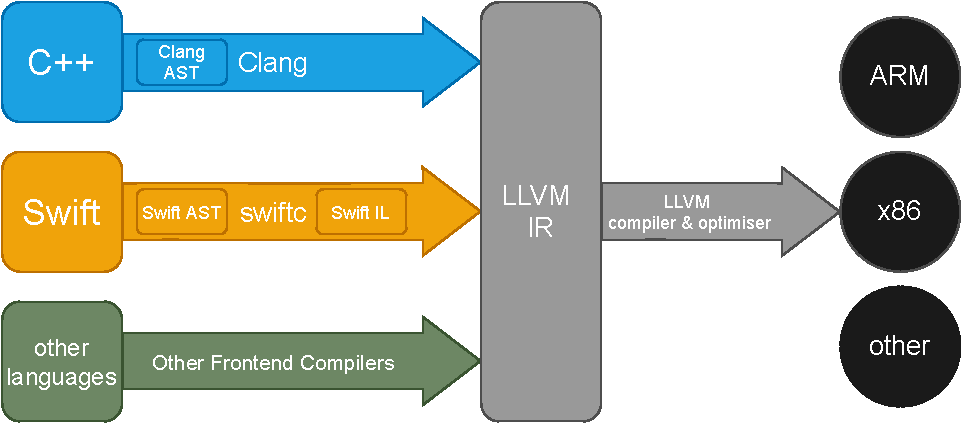
\includegraphics[scale=0.75]{images/llvm.pdf}
        \caption{LLVM design diagram showing how language front-ends create LLVM IR that can be optimised and then used by an architecture back-end, such as x86 to create a machine code executable.}
        \label{fig:llvm-design}
    \end{figure*}  
    
    As seen from \autoref{sec:related-work}, much similar research uses Clang and thus LLVM.
    LLVM~\cite{Lattner2004} is a compiler infrastructure project consisting of several compiler and toolchain technologies. 
    
    LLVM is centrally designed around a language independent intermediate representation (IR), which can be created by a number of language front-ends and is used by a number of back-ends to generate machine code. 
    The LLVM IR is a language-independent, static single assignment (SSA)~\cite{Rosen1988} representation of a program.
    Variables in SSA form can only be assigned once, which allows us to efficiently generate definition-usage graphs, and allows for fast and optimised analysis algorithms to be written.
    Programs can then be optimised by applying portable and reusable transformations on the IR.
    
    Any improvement in back-end machine code generation, as well as any new or improved IR optimisations therefore benefit all of the language front-ends.
    It can be seen that this allows for a very modular and powerful design, shown in \autoref{fig:llvm-design}.
    
    Clang~\cite{Lattner2008} is a LLVM language front-end for C, C++ and a variety of other extensions such as OpenGL.
    By using the LLVM infrastructure, it allows for faster and more efficient compilation of C++ compared to existing, older compilers such as the GNU Compiler Collection~\footnote{\url{https://gcc.gnu.org/}} (GCC)~\cite{Lattner2008}.
    However, most importantly for our research, the design of GCC makes it unsuitable for integration in other projects such as analysis tools, whereas Clang allows access to several analysis tools as well as the Clang abstract syntax tree (AST) and parser internals via a standard API such as consumers and visitors~\cite{Duffy2014}.
    
    \begin{figure}
        \centering
        \inputminted{c++}{code/code-to-ast.cpp}
        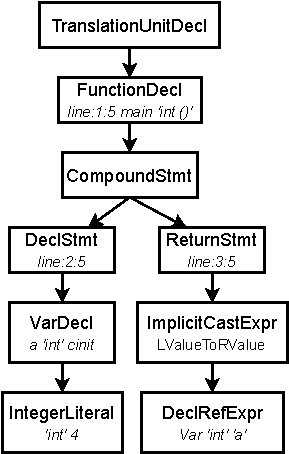
\includegraphics{images/code-to-ast.pdf}
        \caption{Example of converting C++ code to the Clang AST. The Clang AST is rich in information and could be used to reconstruct the original C++ code snippet.}
        \label{fig:code-to-ast-example}
    \end{figure}
    
    Further more, Clang also provides the \emph{LibTooling} C++ library for the creation of tools that leverage the Clang parsing front-end and AST.
    The Clang AST is different from ASTs produced by some other compilers in that it closely resembles the written C++ code~\footnote{\url{https://clang.llvm.org/docs/IntroductionToTheClangAST.html}}.
    For example, we can see in \autoref{fig:code-to-ast-example} that the AST stores much syntactic as well as semantic information in the form of source code locations and variable initialisation styles.
    The LLVM authors remark that this makes it very suitable for refactoring tools.
    
    
%%%%%%%%%%%%%%%%%%%%%%%%%%%%%%%%%%%%%%%%%%%%%%%%%%%%%%%%%%%%%%%%%%%%%%%%%%%%%%%%%%%%%%%%%%%%%%%%%


    \section{Methodology}\label{sec:methodology}
    
    \subsection{Parsing}
    
    The first capability our tool needs is to be able to parse C++ code.
    Doing this ourselves would be an undertaking that would take a significant amount of time in order to create a complete parser due to the size and complexity of the C++ language. Therefore it was decided early to use an existing parser.
    The information in \autoref{subsec:clang-and-llvm} outlines why Clang is the most suitable parser to use, with the other benefits that it brings such as the \emph{LibTooling} library. 
    
    \subsection{Analysis}\label{subsec:methodology-analysis}
    
    Next, our tool would need to be able to identify specifically which pointers are suitable for refactoring into smart pointers.
    An \emph{unique pointer} is a smart pointer that represents a single unique owner of a region of memory at any point in time.
    We will therefore need to develop a static analysis algorithm to identify the maximum number of owners a region of memory has throughout all points of the program. 
    If a memory region has at most a single owner, then we can refactor the initialising raw pointer to be a unique pointer, and otherwise to a shared pointer.    
    This analysis will need to ensure that its result is correct, and will inevitably have to make some conservative assumptions about the program.
    
    \begin{figure}
        \centering
        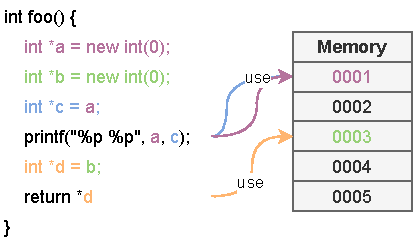
\includegraphics[scale=1.0]{images/memory.pdf}
        \caption{Both the variables \texttt{a} and \texttt{c} end up pointing to memory address \texttt{0001}. Similarly variables \texttt{b} and \texttt{d} point to address \texttt{0003}. The memory at \texttt{0001} is used through two different pointers on line 5, meaning that it is not uniquely owned by a single owner. However, address \texttt{0003} does have a unique single owner at any time in the program, shown by the single incoming arrow to the memory region. Therefore the initialisation of variable \texttt{d} can be modelled as an ownership transfer from \texttt{b}}
        \label{fig:memory-pointers}
    \end{figure} 
    
    A key intuition is that a region of memory, subsequent to its initialisation, is only able to gain additional owners if access to the region of memory is \emph{shared} to another variable, that is if a pointer to this memory is copied to a another pointer, at which point the original owner is no longer the unique owner.
    If we copy the pointer to a global variable, the variable could suddenly be read by any other running threads in the program, so we have to take a conservative decision that the memory no longer has a single unique owner.
    If we copy the pointer to a local variable, then if the original variable remains in use, the memory will have two unique owners. 
    However if the original pointer is not used beyond being copied, this could actually be modelled as a \emph{transfer} of ownership, and the memory will still have a single unique owner at all points of the program. 
    We show this intuition in \autoref{fig:memory-pointers}, where the memory region \texttt{0001} is not suitable for being managed by a unique pointer, whilst region \texttt{0003} is.
    
    We can formalise our key intuition by introducing the concept of \emph{escape analysis}.
    Escape analysis is used to determine whether an object \emph{escapes} or is accessible from outside the method or thread that created the object~\cite{Choi1999}.
    It has been used in languages such as Java~\cite{Choi1999} to determine whether an object which is created within a method escapes.
    If it does not escape, meaning it is only used locally in the method, then the object can be allocated on the stack rather than the heap as a performance optimisation.
    LLVM also uses escape analysis for a similar kind of optimisation~\footnote{\url{https://github.com/llvm/llvm-project/blob/main/llvm/lib/Analysis/CaptureTracking.cpp}}.
    
    It is now apparent that the invariant of the unique pointer is only violated when:
    \begin{itemize}
        \item a pointer escapes, as then we do not know where or how the pointer may be used, so we must take a conservative approach and assume the memory region no longer has at most a single unique owner.
        \item a pointer does not escape but access to the memory is shared rather than transferred between local variables. 
    \end{itemize}
    
    \subsection{Analysis Target}\label{subsec:methodology-analysistarget}
    
    The existing escape analysis in LLVM is implemented to operate on LLVM IR code, as the IR representation, as mentioned in \autoref{subsec:clang-and-llvm}, is well suited for efficient analysis algorithms. 
    However, much of the existing work in \autoref{sec:related-work} use Clang and the Clang AST to perform their parsing, analyses and their source code refactoring..
    We however propose an improved novel design which uses the Clang AST for parsing and refactoring and the LLVM IR for efficient analysis.
    
    For the same input file, we can use the \emph{LibTooling} library to generate an AST and IR in-memory representation.
    Then, for any variable declaration (\texttt{VarDecl}) in the Clang AST which allocates new memory on the heap, we locate this declaration in the IR.
    This is possible as we can instruct Clang to not discard variable names using a \texttt{fno-discard-value-names} flag, and as the combination of function signature and variable name in the translation unit must be unique according to the One-definition rule~\cite{C++17}. 
    
    \begin{listing}
        \inputminted{llvm}{code/code-to-ir.ll}
        \caption{The LLVM IR module representation of the C++ code in \autoref{fig:code-to-ast-example}. Listing has been summarised for clarity. The variable on line 5 can be matched to the variable \texttt{a} in \autoref{fig:code-to-ast-example} by matching the function signature and variable name.}
        \label{lst:code-to-ir}
    \end{listing}
    
    In \autoref{fig:code-to-ast-example}, given the variable declaration for the variable \texttt{a}, then as it is not a global variable, we can visit its parent nodes in the AST until we reach a \texttt{FunctionDecl}.
    We can then use the name of the \texttt{FunctionDecl} to find the corresponding function declaration in the IR module, which can be seen in  \autoref{lst:code-to-ir}.
    Note that although the \texttt{main} function name corresponds exactly, other function names in the IR module will have mangled names~\footnote{\url{https://www.ibm.com/support/knowledgecenter/en/ssw_ibm_i_72/rzarg/name_mangling.html}}.
    We again use Clang library functions to mangle function names if necessary so they can be found in the IR. 
    Given the IR function declaration, we can find the corresponding IR value of our initial variable \texttt{a} by finding the name of the variable inside its symbol table.
    This IR value can then be used to perform our analysis.

    \subsection{Choice of Escape Analysis Algorithm}
    
    The initial choice of escape analysis algorithm is the existing LLVM algorithm mentioned in \autoref{subsec:methodology-analysis}.
    As it is already developed for use on LLVM IR, it is therefore trivial to integrate into the tool which allows us to quickly create a minimal viable product. 
    This allowed for rapid successful prototyping of the tool and therefore reduces risk of the chosen design being unsuitable by following rapid development processes~\cite{Martin1991}.
    We show in \autoref{subsec:methodology-systemdesign} that the design of our tool means that the initial choice of algorithm will not place a limit on the final accuracy or power of the tool.
    
    Investigation of the algorithm shows that it is a conservative analysis with some limits on the analysis complexity so that it does not greatly increase Clang compilation time.
    The analysis uses the definition-usage graph of the value being analysed to add all the instructions that use the value to a work queue.
    Each item in the work queue is then processed and the algorithm dispatches on the type (\emph{opcode}) of the IR instruction.
    It is then checked whether each instruction within the context that it is being used in could cause the value to escape.
    The key limitation that we see of this algorithm is that it is a intraprocedural analysis.
    Pointers are very often used across function boundaries and the conservative decisions the algorithm will take in these situations might limit the effectiveness of the tool in identifying all possible refactoring opportunities. 

    \subsection{Source code rewriting}
    
    The analysis gives a result of whether the IR value escapes, a boolean \texttt{true} or \texttt{false}.
    For a \texttt{false} result, meaning the value does not escape, the variable declaration is refactored into a unique pointer, and otherwise a shared pointer.
    However, the rewriting of the source code is identical for both cases with just the string tokens that replace the original source code differing.
    The rewriting was developed using a rule based approach, using test driven development (TDD) as this allowed rapid but correct development by continuously being able to check that additional created rules still cause all the tests to pass, causing no regressions. 
    The five cases of code (\emph{or the rewriting rules}) that needs to be rewritten are:
    \begin{itemize}
        \item The type of a variable declaration
        \item Variable initialisation or assignment expressions.
        \item Pointer delete statements.
        \item Function return types.
        \item Function call expressions that expect raw pointers.
    \end{itemize}
    
    Rewriting the type of a variable declaration is the easiest of all. We can directly replace the type of the variable declaration node that we already have access to. 
    For example for \mintinline{c++}{int *ptr}, we can extract the type of the variable, and format it into the string \mintinline{c++}{"std::shared_ptr<{}>"} or \mintinline{c++}{"std::unique_ptr<{}>"}, where \texttt{\{\}} represent the replacement field, which in this case will be formatted with the string \mintinline{c++}{int}.
    
    Initialisation and assignment expressions are less simple due to two reasons.
    First of all, the initialisation of a variable does not necessarily have to occur immediately at the point of declaration.
    Therefore we need to find all the points of initialisation or value assignment to a variable in the AST.
    Secondly, there are many different ways to initialise a variable~\cite[p.~196]{C++17}, with the most common initialisation methods using:
    \begin{itemize}
        \item Braced-lists \mintinline{c++}{std::string s{}}.
        \item Equal sign \mintinline{c++}{std::string s = "hello"}
        \item parentheses expression list \mintinline{c++}{std::string s("hello")} 
    \end{itemize}
    For pointer variables, this is convoluted even more depending on if the pointer gets initialised using an existing pointer \mintinline{c++}{int* a = nullptr; int *b = a;}, or if it gets initialised using a \mintinline{c++}{new} statement \mintinline{c++}{auto p = new Circle{Point{0,0},10}}.
    In the case of a new statement, we can initialise the rewritten smart pointer using a value initialiser \mintinline{c++}{std::make_unique<>()} or the shared pointer equivalent. 
    Otherwise, we can initialise the rewritten smart pointer from an existing pointer by using the default equal sign copy initialiser or parentheses expression list. 
    
    Rewriting pointer delete statements also requires us to traverse the AST to find \mintinline{c++}{delete} statements for the variable declaration node that we are rewriting.
    However, this does not require any complicated logic and we can upon finding relevant \mintinline{c++}{delete} statements simply remove them from the source code.
    
    If the variable declaration is a variable that gets returned at the end of the function, then the return type of the function signature will need to be rewritten too. 
    We explicitly check for each variable declaration that we handle if it gets returned, and if so, we can rewrite the function return type the same way that we handle the types of variable declarations.
    
    Lastly, smart pointers have overloaded operators for the arrow \texttt{->} and dereference \texttt{*} operators so that they behave identically as if the value was a raw pointer.
    This simplifies our task as it reduces the amount of rewriting we have to do for each use of the new smart pointer.
    However, there is no such overloaded operator for passing smart pointers as function arguments. 
    In this case, the compiler will find a type error as it might expect a type such as \mintinline{c++}{int *}, but actually receives \mintinline{c++}{std::unique_ptr<int>}. 
    Therefore, we again have to traverse the AST to find all function call expressions which involve the current variable declaration and add \mintinline{c++}{get()} calls in order to get a raw pointer to the managed object.
    We use the \emph{Clang Rewriter}\footnote{\url{https://clang.llvm.org/doxygen/classclang_1_1Rewriter.html}} class as a high level abstraction compared to handling files and text buffers ourselves.
    
    \begin{figure}
        \centering
        \begin{minted}{c++}
        char *test() {
            char* a = new char[2];
            a[0] = 'a';
            printf("\%s", a);
            return a;
        }
        \end{minted}
        
        
\includegraphics{images/arrow.pdf}
        
        \begin{minted}{c++}
        std::shared_ptr<char[]> test() {
            std::shared_ptr<char[]> a = std::shared_ptr<char[]>(new char[2]);
            a.get()[0] = 'a';
            printf("\%s", a.get());
            return a;
        }
        \end{minted}
        
        \caption{An example of all the rewriting rules except pointer delete statements. This example solely shows rewriting and does not necessarily respect any smart pointer viability analyses. We see how both the declaration and equal sign copy initialisation of \texttt{a} have been rewritten to into a \texttt{shared\_ptr}. All the uses of \texttt{a}  that require a raw pointer have a \texttt{get()} call added to obtain the managed memory.}
        \label{fig:rewriting}
    \end{figure}
    
    In \autoref{fig:rewriting}, we show an example that incorporates all the cases in which code needs to be rewritten except pointer delete statements.
    It is visible how in the majority of cases, the first two rules will always be applicable as every new smart pointer needs to have the correct type and be initialised to an object of the right type.
    The fifth rule will also likely be applicable in most cases as variables tend to not be
    unused and therefore will be used in functions that are expecting a raw pointer.
    
    \subsection{System Design}\label{subsec:methodology-systemdesign}
    
    \begin{figure*}
        \centering
        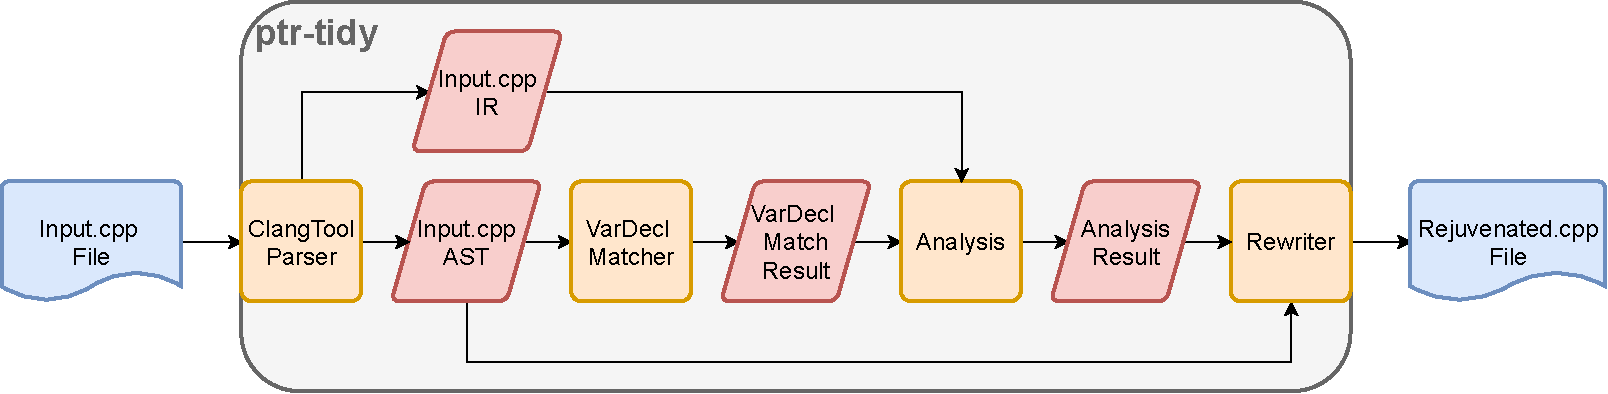
\includegraphics[scale=0.65]{images/design.pdf}
        \caption{System design diagram of the ptr-tidy tool.}
        \label{fig:system-design}
    \end{figure*}
    
    We show the full system design diagram in \autoref{fig:system-design}, showing the full sequence of operations that are executed in order to transform and refactor the input file containing raw pointers into the output file that uses smart pointers.
    The input file is parsed into a Clang AST, which is traversed to find variable declarations.
    The corresponding variable declaration is found in the IR, and used as input to the analysis algorithm.
    The output of the analysis is used in the rewriting component, after which all the changes made in rewriting the program are consolidated and output as the new, improved program.
    
    We believe this design is noteworthy as it closely follows the system design of the general LLVM infrastructure in \autoref{fig:llvm-design}, by having a Clang parser front-end, an analysis middle-end, and a rewriter back-end.
    We also roughly follow the pipeline architectural design, as described by \citet{Schmidt2013}, by having a series of transformation steps, which each have an input and one or more outputs.
    A series of transformation steps are composed until we obtain our end output file.
    This allows us to conform to the Single-responsibility principle as proposed by \citet{Martin2002}.
    This gives us a highly flexible design where different analysis algorithms can be very easily added and trialled for the analysis component, meaning that potentially more powerful analyses can be tested without needing any changed to the parsing or rewriting components. 
    Similarly, given that our analysis is executed on the language-agnostic LLVM IR, the analysis component could be reused by rejuvenation tools for any other languages, allowing our work to be used in future research.

%%%%%%%%%%%%%%%%%%%%%%%%%%%%%%%%%%%%%%%%%%%%%%%%%%%%%%%%%%%%%%%%%%%%%%%%%%%%%%%%%%%%%%%%%%%%%%%%%


    \section{Evaluation}\label{sec:evaluation}
    
    Through our research, we would like to answer the question of whether our implemented tool can truly improve C++ code by seeing if the tool can be used not only on small test examples but also on larger existing programs. We would also like to determine if the rejuvenation produces code which can be compiled and can be judged to be better.
    Then, if the tool is able to do this, we want to evaluate how well the tool performs by analysing the effectiveness of the analysis algorithms.

    In order to evaluate the objectives above, hypotheses were formed:
    
    \begin{itemize}
        \item \textbf{Hypothesis 1} The automatic translation of raw pointers into smart pointers can be used to make existing C++ code more modern and safe.
        \item \textbf{Hypothesis 2} The tool can reliably identify situations in which unique pointers should be used.
    \end{itemize}
    
    Each of these hypotheses will require experimentation to be verified.
    We will answer hypothesis 1 through a case study and we will answer hypothesis 2 through the gathering of relevant metrics on several more projects.
    This section will detail the justification, process, and results for these experiments.
    
    We run our experiments on a Windows 10 Pro x64 machine using the Windows Subsystem for Linux, with an AMD Ryzen 5 PRO 4650U and 16 GiB RAM.
    The ptr-tidy tool was compiled with GCC v10.2.0 using CMake release profile, using Clang and LLVM v11.1.0 libraries.

    \subsection{TinyXML-2 Case Study}\label{subsec:case-study}
    
    In order to answer hypothesis 1, it was decided to run a case study on a specifically chosen C++ project.
    This was decided as an analysis into a well chosen target project will be able to show relevant success and failure cases of the tool.
    If the impact of the success cases outweighs the faults of the failure cases, then we will be able to judge our hypothesis as being true.
    
    We decided on using the \emph{TinyXML-2}~\footnote{\url{https://github.com/leethomason/tinyxml2}} library as our chosen case study.
    TinyXML-2 is a C++ XML parsing library that can parse an XML document and build from that a Document Object Model that can be read, modified, and saved.
    TinyXML-2 has over three thousand \emph{GitHub stars} which puts it in the top 1\% of projects on the hosting website, which can be used as a rough metric for its popularity and good code quality~\cite{Sanatinia2016}.
    It is also used in the \emph{libigl}~\cite{Libigl} geometry processing library,  which itself is used by a variety of large industry companies.
    It is released under a \emph{zlib} license~\footnote{\url{https://opensource.org/licenses/Zlib}} which allows us to use and alter the software.
    What makes the library a particularly attractive choice is the simplicity of the library.
    The library does not make use of the STL~\cite{C++17}, and therefore most importantly does not make use of smart pointers. 
    The library is also around three thousand lines of code in length, making it large enough to likely have a variety of interesting features to analyse, whilst remaining small enough for manual inspection.
    
    \begin{listing}
        \inputminted{cpp}{code/tinyxml2-example.cpp}
        \caption{Example of a method in the TinyXML-2 library which could be refactored to use smart pointers as it returns an owning pointer to a newly created object.}
        \label{lst:tinyxml-refactor-example}
    \end{listing}
    
    In particular, what makes this suitable for the target of our case study over perhaps other similarly small and simple libraries is that due to parsing varying documents at runtime, the library is particularly heavy in pointer logic and memory allocations.
    We can see in \autoref{lst:tinyxml-refactor-example} an example of a method from the library which would be well suited for refactoring to use smart pointers.
    The heavy use of pointers and memory allocation is what leads us to believe that analysis into this library will generalise well onto other C++ projects.
    
    \subsubsection{Experiment}
    
    \begin{listing}
        \inputminted{json}{code/compile_commands.json}
        \caption{Compilation Database for TinyXML-2}
        \label{lst:tinyxml-compilation-database}
    \end{listing}
    
    We first generate a simple \emph{compilation database}~\footnote{\url{https://clang.llvm.org/docs/JSONCompilationDatabase.html}}, as seen in \autoref{lst:tinyxml-compilation-database}, for the TinyXML-2 library, as this is what our tool uses to resolve compilation options. 
    More complex libraries or applications would have their compilation options and any include and link libraries included in compilation command.
    The user of our tool can easily generate a compilation database for the project that they wish to rejuvenate using their build tool, such as \emph{CMake}~\footnote{\url{https://cmake.org/}}.
    
    We can then run the tool on any file which has a compilation command defined in the compilation database, such as the \texttt{tinyxml2.cpp} file from our chosen library.   
    We include the result of the analysis as debug messages during the running of the tool, in order to aid our evaluation of the case study, such as:
    \begin{minted}{text}
    </home/artem/tinyxml2/tinyxml2.cpp:207:70, col:75> Variable curLineNumPtr escapes
    </home/artem/tinyxml2/tinyxml2.cpp:213:5, col:19> Variable start does not escape
    \end{minted}
    
    The final rejuvenated version of the TinyXML-2 is included as reference~\footnote{\url{https://gist.github.com/a-usov/155e55afc5d375070c52ad3e4da19072}}.
    
    \subsubsection{Results and Discussion}
    
    \begin{listing}
        \centering
        \begin{minted}{c++}
        std::shared_ptr<XMLText>  XMLDocument::NewText( const char* str )
        {
            std::shared_ptr<XMLText>  text = std::shared_ptr<XMLText>( CreateUnlinkedNode<XMLText>( _textPool ));
            text->SetValue( str );
            return text;
        }
        \end{minted}
        \caption{Rejuvenated version of the method in \autoref{lst:tinyxml-refactor-example}. The \texttt{text} variable has been identified as being eligible to be a \texttt{shared\_ptr}. The first, second and fourth of our rewriting rules are applied in this example to the \texttt{text} variable.}
        \label{lst:tinyxml-refactor-example-refactored}
    \end{listing}
    
    We can first and foremost see in \autoref{lst:tinyxml-refactor-example-refactored} the result of the rejuvenation on our candidate method in \autoref{lst:tinyxml-refactor-example}.
    
    We can see that we achieve a similar refactoring as in \autoref{fig:rewriting}. 
    The smart pointer is initialised using the pointer copy initialiser.
    We see identical refactoring in the other \texttt{XMLDocument:New...} methods. 
    
    \begin{figure}
        \centering
        \begin{minted}{c++}
        XMLAttribute* XMLElement::CreateAttribute()
        {
            TIXMLASSERT( sizeof( XMLAttribute ) == _document->_attributePool.ItemSize() );
            XMLAttribute* attrib = new (_document->_attributePool.Alloc() ) XMLAttribute();
            TIXMLASSERT( attrib );
            attrib->_memPool = &_document->_attributePool;
            attrib->_memPool->SetTracked();
            return attrib;
        }
        \end{minted}
        
        
\includegraphics{images/arrow.pdf}
        
        \begin{minted}{c++}
        std::shared_ptr<XMLAttribute>  XMLElement::CreateAttribute()
        {
            TIXMLASSERT( sizeof( XMLAttribute ) == _document->_attributePool.ItemSize() );
            std::shared_ptr<XMLAttribute>  attrib = std::make_shared<XMLAttribute>();
            TIXMLASSERT( attrib );
            attrib->_memPool = &_document->_attributePool;
            attrib->_memPool->SetTracked();
            return attrib;
        }
        \end{minted}
        \caption{Rejuvenation of the \texttt{CreateAttribute} method. The \texttt{attrib} variable is copy initialised using the default constructor rather than a copy initialisation using an already allocated pointer. Therefore we identified that the new smart pointer can be initialised using the \texttt{make\_shared} function.}
        \label{fig:rewriting-example2}
    \end{figure}
    
    The only case where our tool was able to successfully refactor the TinyXML-2 library to use the recommended and more efficient \texttt{make\_shared}~\footnote{\url{https://isocpp.github.io/CppCoreGuidelines/CppCoreGuidelines\#Rr-make_shared}} function is shown in \autoref{fig:rewriting-example2}.
    We see the reason for this being that the TinyXML-2 uses memory allocation abstractions such as memory pools rather than creating objects directly through their constructors. 
    Such more detailed refactoring would require human effort.
    
    \begin{figure}
        \centering
        \begin{minted}{c++}
        void nonescapingFunc(int *p) {
            *p += 99;
        }
        \end{minted}
        \begin{minted}{llvm}
        ; Function Attrs: noinline nounwind optnone sspstrong uwtable
        define void @_Z15nonescapingFuncPi(i32* %p) #0 {
        entry:
          %p.addr = alloca i32*, align 8
          store i32* %p, i32** %p.addr, align 8
          %0 = load i32*, i32** %p.addr, align 8
          %1 = load i32, i32* %0, align 4
          %add = add nsw i32 %1, 99
          store i32 %add, i32* %0, align 4
          ret void
        }
        \end{minted}
        \caption{C++ and equivalent LLVM IR snippet showing how function arguments are not considered \texttt{noescape} or \texttt{noalias}}
        \label{fig:function-arguments}
    \end{figure}
    
    Not a single function parameter was refactored to use smart pointers, even though parameters are included in the analysis of the program, since the \texttt{VarDecl Matcher} also matches on arguments (\texttt{ParmVarDecl}) as it is a subclass~\footnote{\url{https://clang.llvm.org/doxygen/classclang_1_1ParmVarDecl.html}}.
    Upon investigation, this is largely an issue due memory coherence guarantees in the specification of the language~\cite[p.~66]{C++17}. 
    Function pointer parameters are assumed by default to escape and to possibly be aliased (\textit{the memory could possibly be accessed through a different variable}).
    Therefore by default no parameters will ever be identified by our analysis as non-escaping and will not be refactored.
    We can see this in \autoref{fig:function-arguments}, where the variable \texttt{p} in the generated LLVM IR is not marked as \texttt{noescape} and \texttt{noalias}~\footnote{\url{https://clang.llvm.org/docs/AttributeReference.html\#noalias}}.
    
    If we enable Clang compiler optimisations when generating the IR for the C++ code in  \autoref{fig:function-arguments}, then the compiler can now correctly identify that \texttt{p} cannot escape within the function, giving it a signature in the IR of 
    \mintinline{llvm}{
    (i32* nocapture %p)
    }.
    However this would break the AST to IR correspondence that we established in \autoref{subsec:methodology-analysistarget} as variables that exist in the AST may find themselves optimised and removed from the IR or functions can that exist in the AST may find themselves inlined in the IR. 
    Also, we still do not have non-aliasing guarantees for the variable \texttt{p} so that we know that the object has not escaped before entering the function.
    It is possible to manually mark a variable in the code as being non-captured and non-aliased by adding parameter attributes such as:
    \begin{minted}{c++}
    void nonescapingFunc(__attribute__((noescape)) int * __restrict__ p) {
        *p += 100;
    }
    \end{minted}
    This relies however on the Clang compiler specific implementation of the \texttt{noescape} attribute which does not exist in the GCC compiler, as well as the non-standard, compiler specific implementation of the \texttt{restrict} attribute. 
    Such code therefore is not portable and not standard conforming, making it likely unacceptable for most projects.
    The LLVM escape analysis currently incorrectly identifies parameters with such attributes to still be escaping, as it is a very rarely occurring optimisation case.

    % The automatic generation of such front-end code however could be possible through the integration of Clang compiler optimisations at the runtime of our tool and through related research such as by \citet{Campos2015} for integration into our tool for better performance.
    
    The impact this has on our tool is that the extent of our analysis is not as complete as we would like it to be, however \autoref{lst:tinyxml-refactor-example-refactored} and \autoref{fig:rewriting-example2} show that we can still achieve desirable results through the analysis of local variables. 
    
    The tool is particularly effective at refactoring factory methods~\cite{Gamma1995} such as in \autoref{lst:tinyxml-refactor-example-refactored} and other cases where resources are created at the top rather than at the bottom of the function call stack and passed through return values.
    
    The rejuvenated version of the TinyXML-2 library that the tool produces is not directly compilable into an object file, mainly due to edge cases in the rewriting component, causing syntactically incorrect output code.
    These mainly stem from the use of now outdated C++ practises.
    For example, the initialisation of a pointer using the value \texttt{0}, such as
    \mintinline{c++}{XMLNode* returnNode = 0;} is not recommended as they should be initialised with \mintinline{c++}{nullptr}.
    The rejuvenation of the example into
    \mint{c++}|std::shared_ptr<XMLNode>  returnNode = std::shared_ptr<XMLNode>(0);|
    therefore causes a type error during compilation as the \mintinline{c++}{shared_ptr} constructor has stricter type checking. 
    
    All of the compilation issues currently stem from unimplemented behaviour in the rewriting component rather than the strength or performance of the analysis.
    The size and complexity of the language makes it difficult to ensure that all edge cases are handled by the rewriting component, which can in future development be continuously improved.
    The fixes that need to be applied in order to compile the rejuvenated program can be done manually by the programmer, with all of the identified fixes in the TinyXML-2 library being a single line in length. 
    
    However, we do not think this detracts from the value or usefulness of our tool.
    Our tool provides fully rejuvenated and compilable programs without the need for any human input for simpler input programs. 
    These programs are modernised to use features such as smart pointers, which also bring stricter type checking.
    For larger, more complex and older input programs some human input is currently still needed, however the work of our tool allows the programmer to make their programs more modern and safer by performing the complex analysis and guiding the programmer towards the needed fixes through compiler errors.
    This results in the rejuvenated output being obtained more easily by removing the need for the programmer to manually understand the structure and style of the program and the often complex ownership relations between the various variables in the program. 
    
    We therefore believe that from the analysis of our tool on the case study of the TinyXML-2 library, even with the identified failure cases, the success of the automated translation and identified success cases allow us to confirm our first hypothesis.
    
    \subsection{Analysis of performance on a corpus of projects}
    
    \begin{table*}
        \begin{tabular}{|l|l|l|l|l|l|l|l|l|}
        \hline
                                        & \textbf{clipper} & \textbf{happyhttp} & \textbf{jzon} & \textbf{micropather} & \textbf{poisson} & \textbf{polypartition} & \textbf{tinyxml2} & \textbf{xatlas} \\ \hline \hline
        \textbf{Runtime (ms)}          & 146.521          & 10.540             & 3.140                & 2.429         & 4.471            & 11.885                 & 16.055            & 105.212         \\ \hline
        \textbf{Escaped Pointer}       & 94               & 22                 & 2                    & 39            & 7                & 46                     & 164               & 235             \\ \hline
        \textbf{Non-Escaped Pointers}  & 132              & 16                 & 3                    & 34            & 3                & 22                     & 84                & 111             \\ \hline
        \textbf{Lines of Code Changed}   & 205             & 27                 & 3                    & 57            & 6                & 31                     & 142               & 154             \\ \hline
        \textbf{Total Lines of Code} & 5035             & 1273               & 1324                 & 1587          & 523              & 2270                   & 5366              & 10318           \\ \hline
        \end{tabular}    
        \caption{Data gathered from the rejuvenation of each projects. Total lines of code include both the implementation and header file of each project. Runtime measured in milliseconds as the median of five runs.}
        \label{table:data}
    \end{table*}
    
    \begin{figure*}
        \centering
        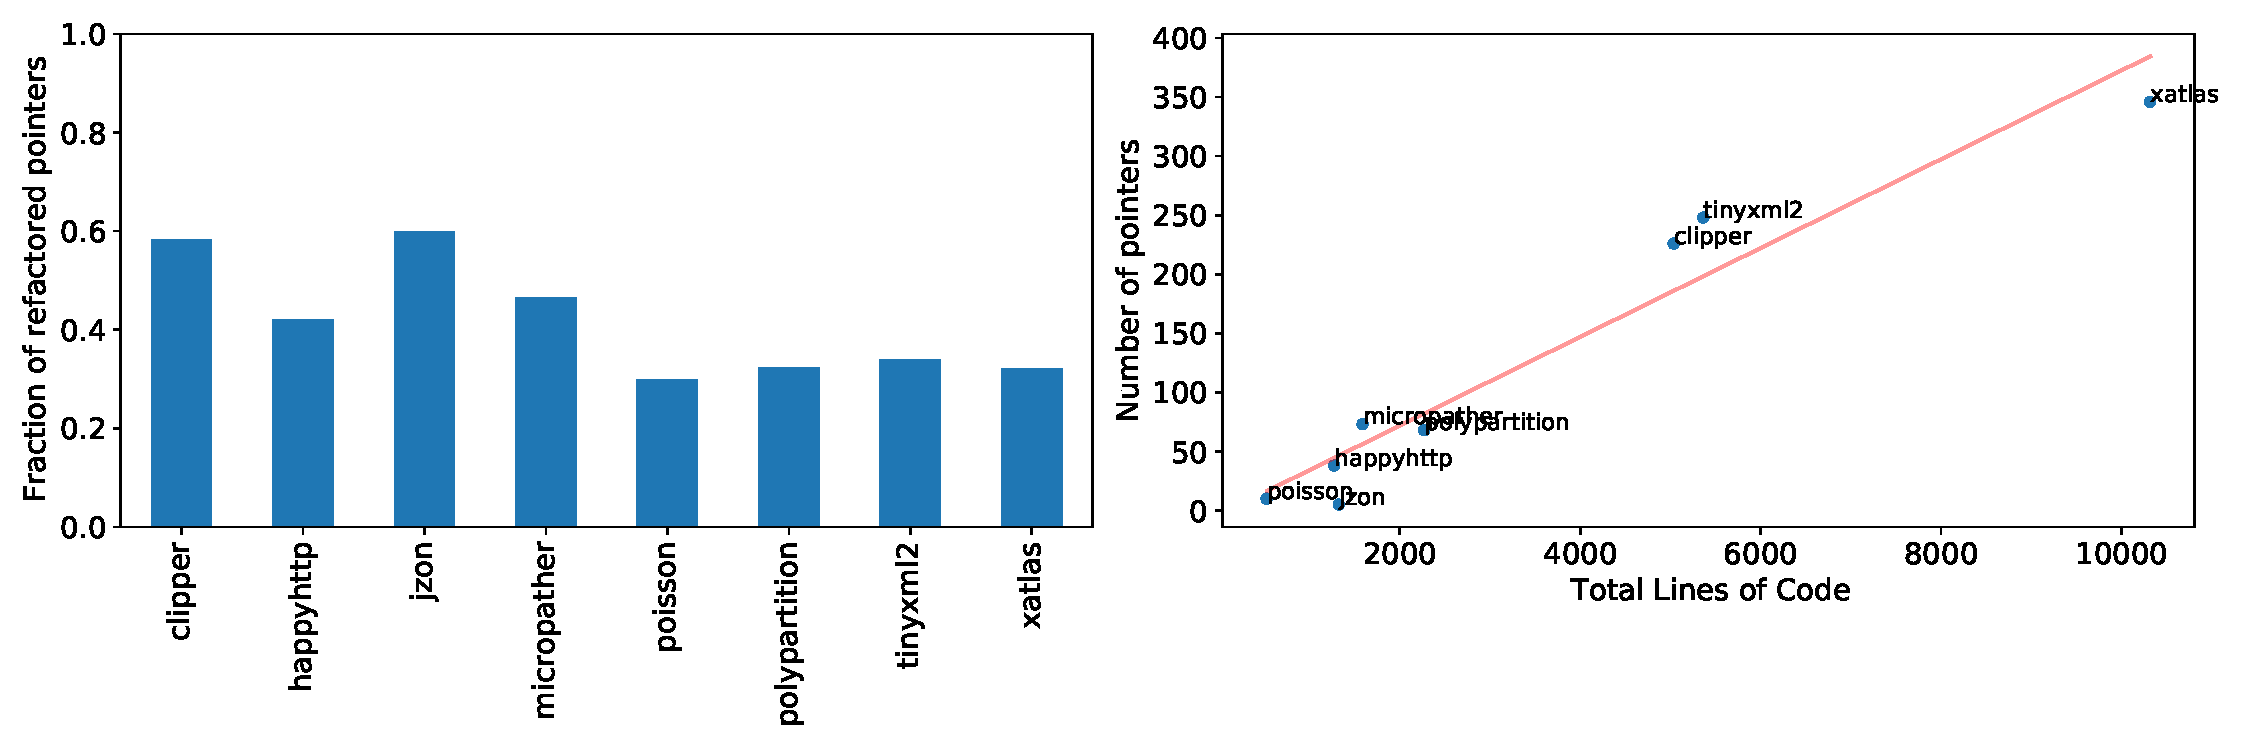
\includegraphics[scale=0.45]{images/pointers.pdf}
        \caption{First graph shows the fraction of non-escaped, and therefore refactored, pointers for each project. This varies from a minimum of 30\% up to a maximum of 60\%, with a mean of 42\%. The second graph shows the number of total pointers compared to the number of total lines in each project.}
        \label{fig:ratio-pointer}
    \end{figure*}
    
    \begin{figure*}
        \centering
        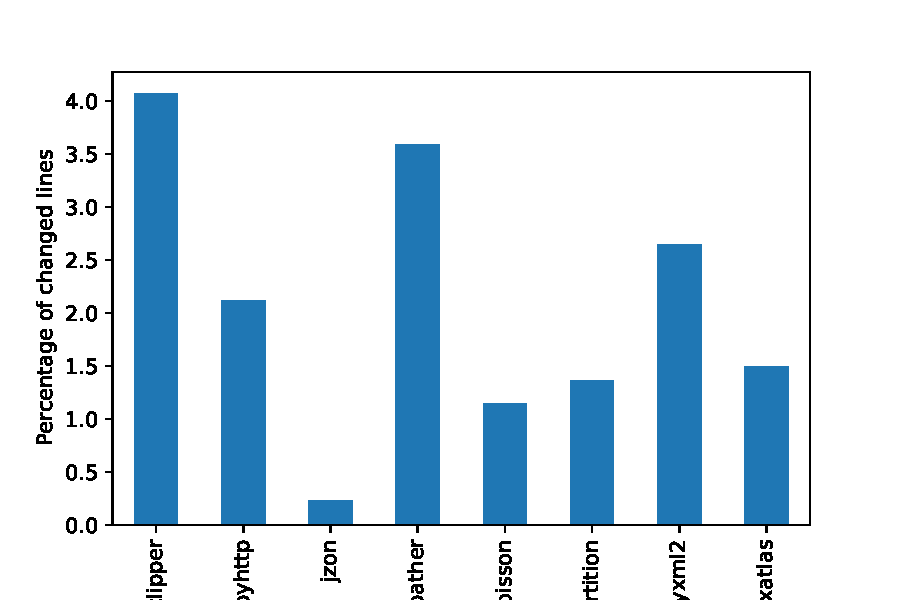
\includegraphics[scale=0.8]{images/lines.pdf}
        \caption{Graph showing the fraction of modified lines by the tool compared to the total number of lines in each project, which is the combination of implementation and header files. This varies from a minimum of 0.22\% up to a maximum of 4.07\%, with a mean of 2.18\%.}
        \label{fig:lines}
    \end{figure*}

    \begin{figure*}
        \centering
        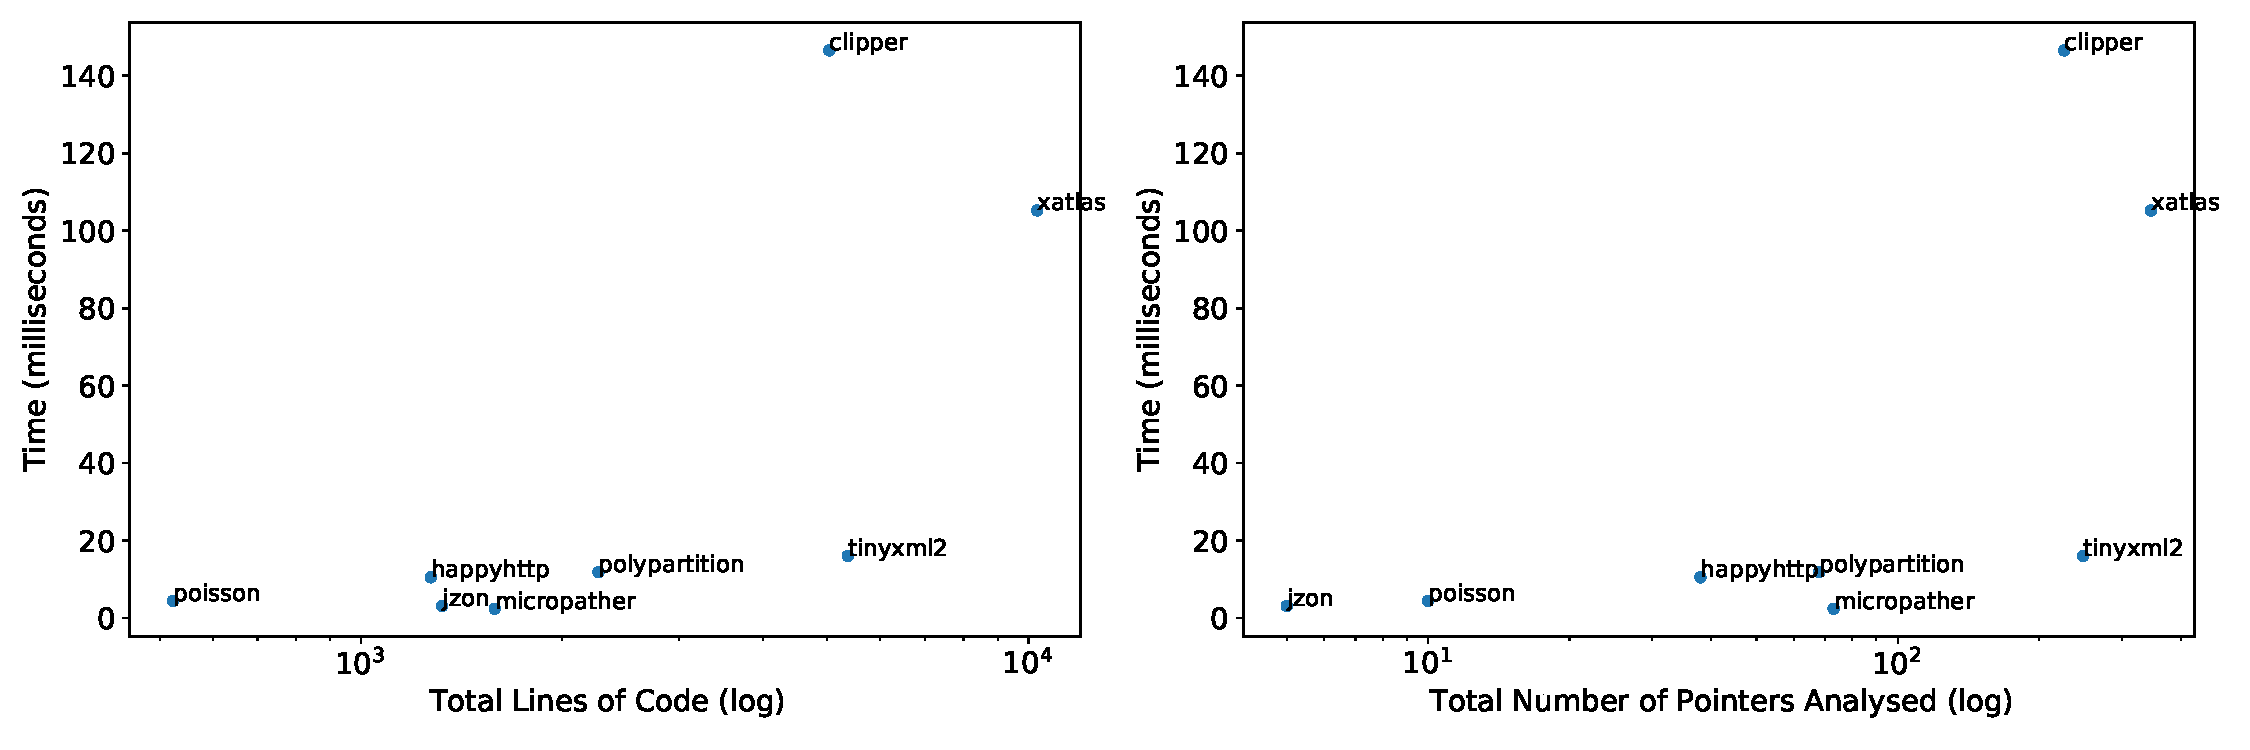
\includegraphics[scale=0.475]{images/time.pdf}
        \caption{Graphs of the tool runtime versus the total lines of code in each project and the total number of pointers that was analysed. The x axis for both graphs are plotted on a log scale. This is for clarity purposes in order to emphasise the two outliers consisting of the Clipper and Xatlas libraries. Time was measured in microsecond using the Bash \texttt{time} command and measured as the median real execution time of 5 runs.}
        \label{fig:time}
    \end{figure*}

    In order to answer hypothesis 2, it was decided to run analysis of the tool on more open source projects and gather metrics on the performance of the tool in terms of its performance in successfully identifying pointers can be refactored, how extensive the rejuvenation is in context of the whole program, and some general runtime characteristics. 
    
    It was decided that whilst gathering more projects to test, we would continue to focus on simple, single file libraries similar to TinyXML-2 in order to ease the cost of setting up each project to be used by the tool. 
    We used a list of single file, public-domain/open source libraries with minimal dependencies~\cite{Barrett2019} by acknowledged game and software developer Sean Barret~\footnote{\url{https://www.mobygames.com/developer/sheet/view/developerId,4966/}} to discover as many as possible candidate libraries.
    This list also ensures that we select projects from many areas of software engineering such as graphics and geometry to file parsers.
    This ensures that we run the tool across a wide variety of projects which will have different distributions and usages of memory allocations and pointer use, giving greater validity that our tool is able to generalise to any type of project.
    We filtered projects from the list that are C++ only, do not already use smart pointers and have at least one dynamic memory allocation and are not header-only.
    With this, we arrived at the following list of selected projects: 
    
    \begin{itemize}
        \item \textbf{Clipper} for clipping and offsetting lines and polygons~\footnote{\url{http://www.angusj.com/delphi/clipper.php}}.
        \item \textbf{HappyHTTP} for issuing HTTP requests and processing responses~\footnote{\url{http://scumways.com/happyhttp/happyhttp.html}}.
        \item \textbf{MicroPather} for path finding and A* solving.~\footnote{\url{http://www.grinninglizard.com/MicroPather/}}.
        \item \textbf{Jzon} for JSON parsing~\footnote{\url{https://github.com/Zguy/Jzon}}.
        \item \textbf{Poisson Disk Points Generator}~\footnote{\url{https://github.com/corporateshark/poisson-disk-generator}}.
        \item \textbf{PolyPartition} for polygon partition and triangulation~\footnote{\url{https://github.com/ivanfratric/polypartition}}.
        \item \textbf{TinyXML-2} for XML parsing~\footnote{\url{https://github.com/leethomason/tinyxml2}}.
        \item \textbf{Xatlas} for generating unique texture coordinates suitable for baking lightmaps or texture painting~\footnote{\url{https://github.com/jpcy/xatlas}}.
    \end{itemize}
    
    We first modified the tool to include a simple counter for how many pointers that are analysed are identified as escaping and how many as non-escaping.
    We also disabled any output of debug messages in order to not skew the tool runtime with writing large amounts of text, other than the output rejuvenated program, as this is the essential function of the tool.
    We measure the runtime of the tool on each project as the median of five runs, on a machine with no other programs running, recording the pointer analysis statistics as well.
    We measure the number of lines changed by using the output of the Linux \texttt{diff} command on the rejuvenated and original files. 
    We show the raw data of the gathered metrics in \autoref{table:data}.
    
    \subsubsection{Results and Discussion}
    
    We see first of all in \autoref{fig:ratio-pointer} that our tool has consistent behaviour across the various projects, with 4 projects having between 30\% and 40\% of pointers identified for refactoring and 4 other projects having between 40\% and 60\% of pointers identified. 
    The mean of 42\% shows that we are able to identify a non-trivial amount of pointers, however it is unclear this is not higher because of a fault in the analysis or whether this is the typical performance for a conservative analysis.
    The second graph in \autoref{fig:ratio-pointer} also shows how the amount of pointers in a project as the size of the project increases is close to linear. 
    This is a surprising result as we expected that different project in different areas of computer science of the same length would utilise vastly different amounts of memory allocations and use vastly different amounts of pointers.
    There seems to be no relationship between the 4 projects that had over 40\% of pointers identified and their lengths.
    We therefore conclude that the size of a project that the tool has to rejuvenate has no impact on its performance. 
    
    \autoref{fig:lines} shows the number of lines that were modified in the rejuvenated version of the project compared to the original. 
    We can much more clearly see our previous expectation that some projects utilise pointers more and other less. 
    The two projects with the lowest amount of modified lines, Jzon and the Poisson Disk Points Generator both only had ten or less pointers to analyse in total, with the Jzon library in particular only having three changed lines from the original. 
    Manual investigation of the Jzon library shows that even though it is a parsing library like TinyXML-2, the amount of code limited to memory allocations and pointers is very minimal. 
    We therefore again conclude that it seems like the tool is able to generalise well to different input programs.
    
    Lastly, \autoref{fig:time} shows two graphs, plotting the runtime of the tool on the selected projects versus the lines of code and number of pointers that they contain.
    Unlike usual refactoring tools, our tool as a rejuvenation tool is only intended to be run once on a code base, compared to a tool such as \texttt{clang-tidy}~\footnote{\url{https://clang.llvm.org/extra/clang-tidy/}} which is usually invoked many times. 
    Therefore, we do not have a strict requirement on a fast processing time. 
    However, we can see that for the majority of projects, the processing remains under twenty milliseconds, even as the number of lines of code increases to over 5000. 
    We see a linear relationship in both of the graphs, except for the outliers of the Clipper and Xatlas libraries.
    We were unable to establish why these libraries take an exceptionally longer time to process, especially since the TinyXML-2 library has a similar amount of lines of code and analysed pointers as the Clipper library. 
    This gives us confidence that the use of our tool would scale well onto even larger projects and therefore as useful as possible.
    
    To conclude, we believe we can partially confirm our second hypothesis.
    We show that the tool generalises to a range of other libraries apart from the TinyXML-2 library selected in our case study and show that our analysis achieves similar results across all these libraries. 
    However, what we cannot conclude is the accuracy of our tool in terms of the best case performance. 
    We were not able to find in the literature an estimate for the fraction of code that is used for memory management, nor are we able to confirm that our analysis achieves the best possible result out of any possible analysis that could be implemented.
    
    
%%%%%%%%%%%%%%%%%%%%%%%%%%%%%%%%%%%%%%%%%%%%%%%%%%%%%%%%%%%%%%%%%%%%%%%%%%%%%%%%%%%%%%%%%%%%%%%%%


    \section{Conclusions}\label{sec:conclusions}
    
    In this paper, we present the problem of \emph{manual memory management} in C++ and how it can create the opportunity for exploitable \emph{memory safety errors}. 
    We show how modern C++, that is the C++ 11 standard and newer, encourage the use of \emph{smart pointers} instead for memory management. 
    Smart pointers create resource handles which automatically get released when the handle exits the scope of a function or method. 
    This referred to as \emph{RAII} (\textit{Resource Acquisition is Initialisation}).
    We also highlight the eventual increasing need for automatic rejuvenation, the replacement of outdated coding patterns with newer, higher-level abstractions, of maintained projects as languages move and evolve much quicker than can be supported in enterprise environments.
    
    We then introduce our \emph{ptr-tidy} tool in order to automatically rejuvenate code that does not use smart pointers, thereby solving our first problem.
    We show the design and implementation of the tool, which uses the Clang and LLVM libraries. 
    The tool uses Clang and the Clang abstract syntax tree (AST) in order to obtain a rich and closely resembling representation of the input program.
    The tool then uses the equivalent representation of the input program in the lower-level LLVM intermediate representation (IR) in order to analyse which pointers are suitable to be \emph{unique pointers} or \emph{shared pointers}. 
    The AST and output of the analysis are then input to a rewriting component which creates and outputs our final rejuvenated program. 
    This design is the solution to our second problem, as we believe this design is both generic, reusable and powerful enough to be used for a variety of rejuvenations.
    The design of the LLVM IR allows for powerful and efficient analyses to be performed, whilst its language agnostic nature allows a variety of possible parsing front-ends and output back-ends to be used, such as existing mature implementations available for C++ or Rust.
    
    Our evaluation showed that our tool can effectively be used to rejuvenate a set of simple open-source libraries, with a specific in depth analysis into the TinyXML-2 library that showed correct rejuvenations in object factory methods. 
    We observe that the tool is particularly effective at rejuvenating specific cases in programs where dynamic resources are created at the top of the function call stack and passed down the stack through return values. 
    We also discovered that due to limitations in the specification of the C++ language, we are unable to rejuvenate function parameters, which meant the extent of our rejuvenation had limits.
    The successful application of the tool across a varied set of open-source projects allowed us to conclude that the analysis and design of the tool were indeed suitable for refactoring generic C++ programs. 
    
    \subsection{Future Work}
    
    The escape analysis algorithm described by \citet{Choi1999} is used as the default escape analysis algorithm in the Oracle Java Virtual Machine implementation~\footnote{\url{https://docs.oracle.com/en/java/javase/16/vm/java-hotspot-virtual-machine-performance-enhancements.html}} and is widely cited~\cite{Wang2020, Stadler2014}.
    Most importantly, the authors present an interprocedural analysis which we hypothesise could bring greater effectiveness to our tool as we believe that it could lead to improved analysis performance compared to our implemented intraprocedural analysis. 
    The similarity of Java and C++ as object oriented languages should allow for a direct application of the algorithm in C++.
    
    Secondly, we mention in \autoref{subsec:case-study} that we are unable to enable optimising compiler invocations for generating the LLVM IR as it breaks our AST to IR correspondence. 
    However, it remains to be investigated whether these optimisations can be called dynamically during the running of our tool in order to gain insight into conservative assumptions that we currently have to make. 
    
    In terms of the evaluation of the tool, we would like to extend it with more complex, multi-file projects and determine whether the translation unit barrier, where an analysis pass can only access the current implementation file, has an impact on analysis performance.
    An inter-modular analysis, similar to existing link time optimisations in compilers~\footnote{\url{https://llvm.org/docs/LinkTimeOptimization.html}}, can then be evaluated whether it brings greater analysis performance. 
    

%%%%%%%%%%%%%%%%%%%%%%%%%%%%%%%%%%%%%%%%%%%%%%%%%%%%%%%%%%%%%%%%%%%%%%%%%%%%%%%%%%%%%%%%%%%%%%%%%


    \vskip8pt \noindent
    \textbf{Acknowledgements.}
    
    I would like to thank my supervisor Dr Jeremy Singer for his guidance and feedback throughout the duration of the project.
    I would also like to thank my family for their continued support.

    \bibliographystyle{abbrvnat}
    \bibliography{paper}

\end{document}
